\documentclass[eng,openany]{mgr}
\usepackage{listings}
\usepackage[english]{babel}
\usepackage{graphicx}
\usepackage{hyperref}
\usepackage{tabularx,colortbl} 
\usepackage{rotating}
\usepackage[utf8]{inputenc} 
\setlength\parindent{24pt}
\usepackage[parfill]{parskip}
\usepackage[table,kernelfbox,hyperref]{xcolor}
\usepackage{fancyhdr}
\usepackage{gauss}
%\usepackage[colorinlistoftodos]{todonotes}

\hypersetup{colorlinks=true}
\hypersetup{xurlbordercolor=red!70!black}
\hypersetup{xlinkbordercolor=blue!70!black}
\hypersetup{linkcolor=blue!60!black}
\hypersetup{urlcolor=red!50!black}
\hypersetup{citecolor=green!30!black}
\rfoot{Page \thepage}
\renewcommand\lstlistlistingname{List of Listings}
\newcommand{\linia}{\rule{\linewidth}{0.4mm}}

\definecolor{listlightgray}{gray}{0.93}

\newcommand{\lstsetmylst} {
\lstset{frame = tb,
breaklines=true,
framerule = 0.25pt,
float,
fontadjust,
backgroundcolor={\color{listlightgray}},
basicstyle = {\ttfamily\footnotesize},
identifierstyle = {\ttfamily},
stringstyle = {\ttfamily},
showstringspaces = false,
showtabs = false,
numbers = left,
numbersep = 6pt,
tabsize = 4,
language=C,
floatplacement=!h
}
}

\newcommand{\lstsetatc} {
\lstset{frame = tb,
breaklines=true,
framerule = 0.25pt,
float,
fontadjust,
backgroundcolor={\color{listlightgray}},
basicstyle = {\ttfamily\footnotesize},
keywordstyle = {\ttfamily\color{listkeyword}\textbf},
identifierstyle = {\ttfamily},
commentstyle = {\ttfamily\color{listcomment}\textit},
stringstyle = {\ttfamily},
showstringspaces = false,
showtabs = false,
numbers = left,
numbersep = 6pt,
numberstyle={\ttfamily\color{listnumbers}},
tabsize = 4,
language=C,
floatplacement=!h
}
}

\newcommand{\lstsetatbashnum} {
\lstset{frame = tb,
breaklines=true,
framerule = 0.25pt,
aboveskip=2ex,
float,
fontadjust,
backgroundcolor={\color{listlightgray}},
basicstyle = {\ttfamily\footnotesize},
keywordstyle = {\ttfamily\color{listkeyword}\textbf},
identifierstyle = {\ttfamily},
commentstyle = {\ttfamily\color{listcomment}\textit},
stringstyle = {\ttfamily},
showstringspaces = false,
showtabs = false,
numbers = left,
numbersep = 6pt,
numberstyle={\ttfamily\color{listnumbers}},
tabsize = 4,
language=bash,
floatplacement=!h
}
}
\lstsetmylst
\author{Jaroslaw M. Szumega}
\title{}
\engtitle{}
\supervisor{Rafal Zdunek, D.Sc, K-4/W4}
\field{Electronics}
\specialisation{Advanced Applied Electronics}
\date{08.06.2017}
\begin{document}
\selectlanguage{english}
\maketitle
\tableofcontents
\newpage

\chapter{Solution to the given problems}
\begin{figure}[h]
\centering

\includegraphics[width=0.7\linewidth]{screenshot001}
\label{fig:screenshot001}
\end{figure}
\begin{figure}[h]
\centering
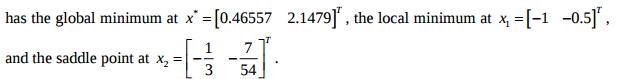
\includegraphics[width=0.7\linewidth]{screenshot002}
\label{fig:screenshot002}
\end{figure}


In general, the unconstrained nonlinear least squares problem is equivalent to:
\begin{flalign*}
\min_{x} \sum_{i=1}^N F_i^2(x)
\end{flalign*}
with the objective function:
\begin{flalign*}
f(x) = \frac{1}{2} \sum_{i=1}^N F_i^2(x)
\end{flalign*}

In the case of the following task, objective function will be
\begin{flalign*}
f(x) &= \frac{1}{2}(F_1^2 + F_2^2)\\
&= \frac{1}{2}[(x_1^6 + 6x_1^5 + 15x_1^4 - 2x_1^3x_2 + 18x_1^3 - 6x_1^2x_2 + 9x_1^2 - 6x_1x_2 + x_2^2)\\
&+\ \ \ 
(x_1^4 + 4x_1^3 - 2x_1^2x_2 + 6x_1^2 - 4x_1x_2 + 4x_1 + x_2^2 - 2x_2 + 1)]\\
&= \frac{1}{2}(x_1^6 + 6x_1^5 + 16x_1^4 - 2x_1^3x_2 + 22x_1^3 - 8x_1^2x_2 + 15x_1^2 - 10x_1x_2 + 4x_1 + 2x_2^2 - 2x_2 + 1)
\end{flalign*}
\\
And the points to check are:\\
\begin{flalign*}
x^* &= [0.46557\ 2.1479]^T\\
x_1 &= [-1\ -0.5]^T\\
x_2 &= [-\frac{1}{3}\ -\frac{7}{54}]^T
\end{flalign*}
\\
Firstly, we can calculate the cost function gradient to verify above--mentioned points:

\begin{flalign*}
\nabla f(x^*) &= 0\\ \\
\frac{\delta f(x)}{\delta x_1} &= 3 x_{1}^{5} + 15 x_{1}^{4} + 32 x_{1}^{3} - 3 x_{1}^{2} x_{2} + 33 x_{1}^{2} - 8 x_{1} x_{2} + 15 x_{1} - 5 x_{2} + 2\\
\frac{\delta f(x)}{\delta x_2} &= - x_{1}^{3} - 4 x_{1}^{2} - 5 x_{1} + 2 x_{2} - 1\\
\end{flalign*}

And in fact, the mentioned in task description points are recognized as a solutions of the cost function gradient.\\
\\
To check their nature, we need to calculate the Hessian and evaluate it according to the stationary points.
\begin{flalign*}
\nabla^2 f(x)\ &= 
\begin{bmatrix}%
\frac{\delta^2 f(x)}{\delta x_1^2} & \frac{\delta^2 f(x)}{\delta x_1x_2}\\
\frac{\delta^2 f(x)}{\delta x_1x_2} & \frac{\delta^2 f(x)}{\delta x_2^2}
\end{bmatrix}\\
\end{flalign*}
\begin{math}
\nabla^2 f(x)\ = 
\begin{bmatrix}%
15 x_{1}^{4} + 60 x_{1}^{3} + 96 x_{1}^{2} - 6 x_{1} x_{2} + 66 x_{1} - 8 x_{2} + 15& - 3 x_{1}^{2} + 8 x_{1} + 5\\
- 3 x_{1}^{2} + 8 x_{1} + 5& 2
\end{bmatrix}\\
\end{math}

\begin{flalign*}
for\ point\ [0.46557\ 2.1479] &=
\begin{bmatrix}%
50.11& -9.37\\
-9.37&2\\
\end{bmatrix}\\
det > 0, M1 > 0, f(x) = 5.01e-11, &\ there\ is\ a\ minimum\ (global)
\\
\\
for\ point\ [-1\ -0.5] &=
\begin{bmatrix}%
1& 0\\
0&2
\end{bmatrix}\\
det > 0, M1 > 0, f(x) = 0.25, &\ there\ is\ a\ minimum
\\
\\
for\ point\ [-\frac{1}{3}\ -\frac{7}{54}] &=
\begin{bmatrix}%
2.41&-2.66\\
-2.66&2\\
\end{bmatrix}\\
det < 0, M1 > 0, f(x) = 0.33, &\ there\ is\ a\ saddle\ point
\end{flalign*}


To make all the calculations above, the following script in Python was written to perform symbolic computations:
\newpage
\begin{lstlisting}
#!/usr/bin/python

from sympy import diff, Symbol, latex, Matrix


def optimization(function, x1, x2):

	print latex(function)
	
	#calculating the gradient's elements
	firstx1 = diff(function, x1)
	firstx2 = diff(function, x2)
	
	print firstx1.expand()
	print firstx2.expand()
	
	
	#calculations for Hessian elements
	secondx1x1 = diff(function, x1, x1)
	secondx1x2 = diff(function, x1, x2)
	secondx2x1 = diff(function, x2, x1)
	secondx2x2 = diff(function, x2, x2)
	
	print "\n Hessian elements:\n\n"
	print latex(secondx1x1) +"\t" + latex(secondx1x2)
	print latex(secondx2x1) + "\t"+latex(secondx2x2)
	
	
	point1 = [0.46557, 2.1479]
	point2 = [-1.0, -0.5]
	point3 = [-1.0/3, -7.0/54]
	
	point = point3
	print secondx1x1.subs(x1, point[0]).subs(x2, point[1]);
	print secondx1x2.subs(x1, point[0]).subs(x2, point[1]);
	print secondx2x1.subs(x1, point[0]).subs(x2, point[1]);
	print secondx2x2.subs(x1, point[0]).subs(x2, point[1]);
	print "\n\n"
	print function.subs(x1, point[0]).subs(x2, point[1]);	


def main():
	x1 = Symbol('x1')
	x2 = Symbol('x2')
	
	f1 = x1**3 + 3*x1**2 + 3*x1 - x2
	f2 = x1**2+2*x1 -x2 + 1
	f = (f1**2 + f2**2)/2	
	
	function = f.expand()
	optimization(function, x1,x2)

main()
\end{lstlisting}
\newpage

%task2
\begin{figure}[h]
\centering
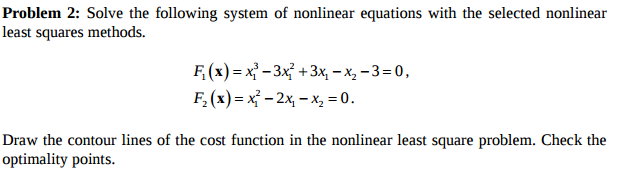
\includegraphics[width=0.7\linewidth]{screenshot003}
\label{fig:screenshot003}
\end{figure}

To resolve this nonlinear LS problem, the Newton and Broyden algorithm were used.
\begin{lstlisting}
Newton's Method
iteration =  5

x =
2.4656	1.1479

Elapsed time is 0.000832081 seconds.


Broyden Method
iteration =  424

x =
2.4656 1.1479

Elapsed time is 0.055002 seconds.
\end{lstlisting}


\begin{figure}[h]
\centering
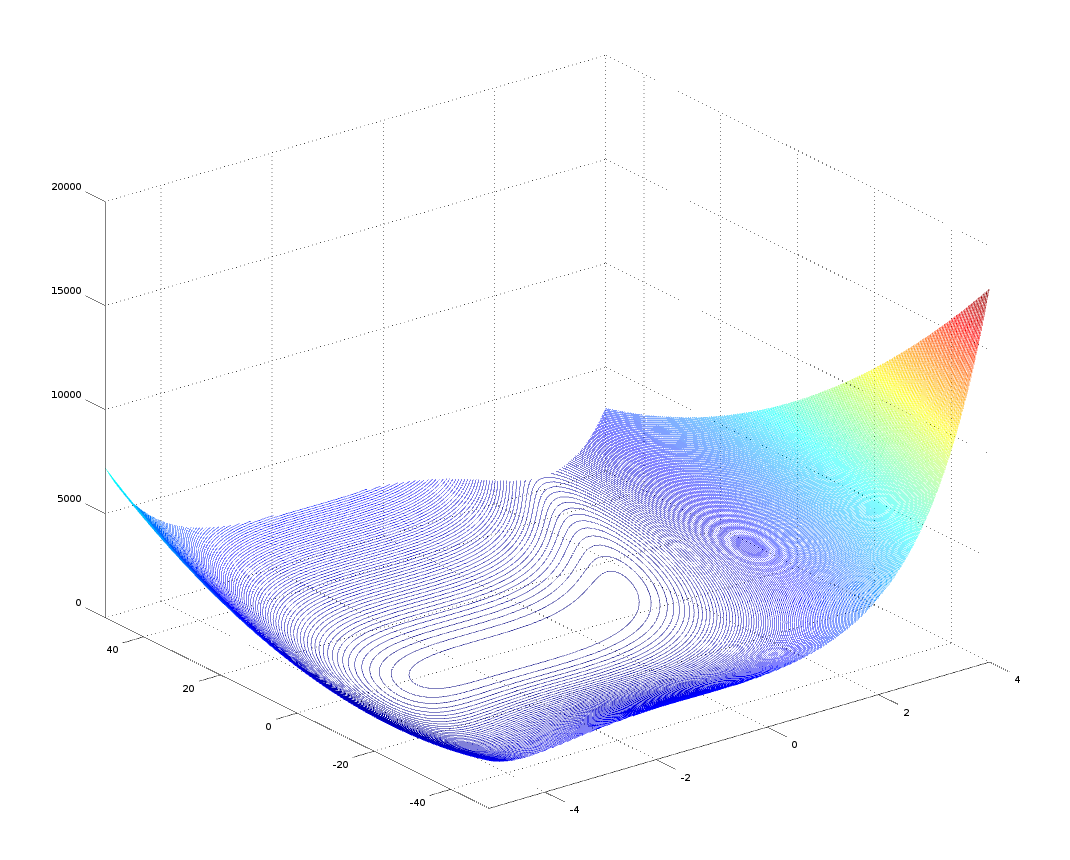
\includegraphics[width=0.7\linewidth]{screenshot004}
\caption{Contour plot of cost function.}
\label{fig:screenshot004}
\end{figure}
\clearpage



%task3
\begin{figure}[h]
\centering
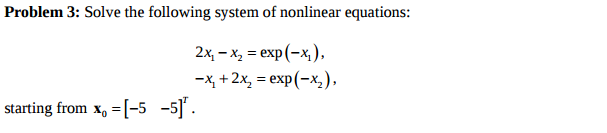
\includegraphics[width=0.7\linewidth]{screenshot005}
\label{fig:screenshot005}
\end{figure}
\begin{lstlisting}
Newton Method
x =
0.56714
0.56714

iter_newton =  8
Elapsed time is 0.00742817 seconds.


Broyden Method
x =
0.56714
0.56714

iter_broyden =  8
Elapsed time is 0.00764704 seconds.
\end{lstlisting}
\begin{figure}[h]
\centering
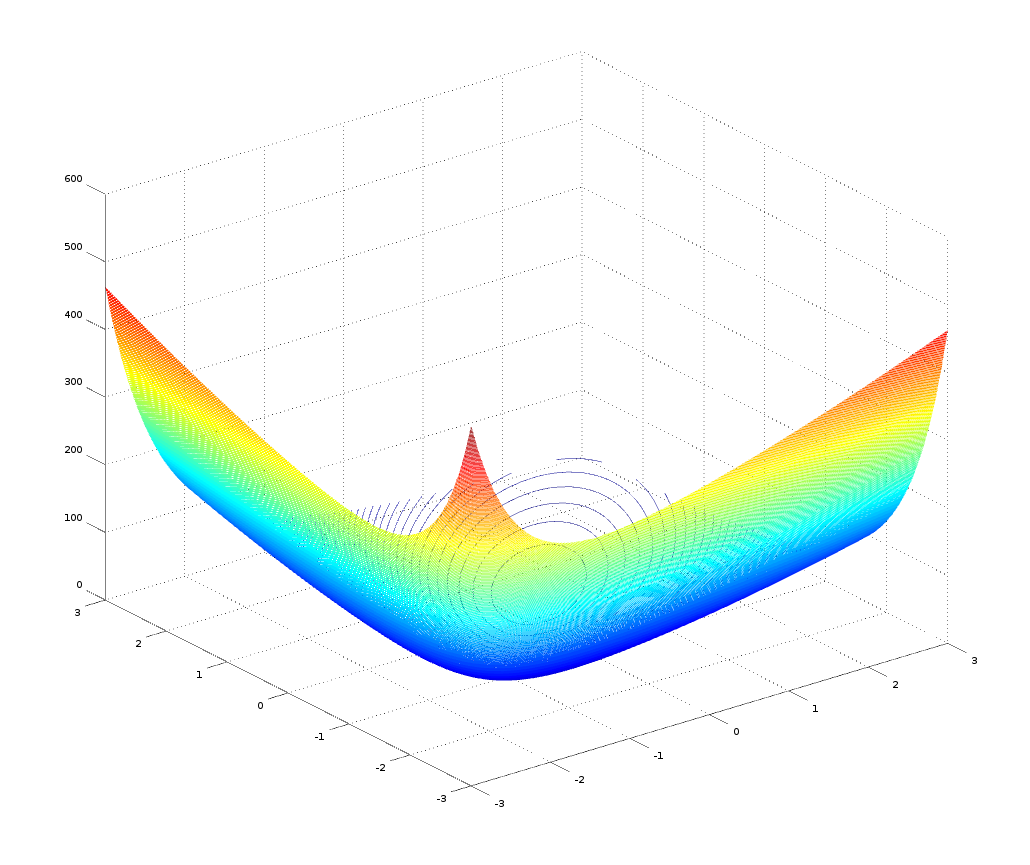
\includegraphics[width=0.7\linewidth]{screenshot006}
\caption{Contour plot of cost function}
\label{fig:screenshot006}
\end{figure}
\clearpage




%task4
\begin{figure}[h]
\centering
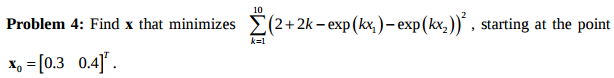
\includegraphics[width=0.7\linewidth]{screenshot007}
\label{fig:screenshot007}
\end{figure}
To complete this task, the \textbf{lsqnonlin} function was used.\\
In order to make this experiment more interesting, here will be shown its usage in two ways:
\begin{itemize}
	\item without using Jacobian calculations,
	\item with Jacobian calculations. It will be turned on using Octave options.
\end{itemize}
There fore there was prepared two versions of evaluation function to pass to the lsgnonlin:\begin{lstlisting}
function [F,J] = fun_4(x)
	k = 1:10;
	F = 2 + 2*k-exp(k*x(1))-exp(k*x(2));
endfunction

function [F,J] = fun_4_Jacobian(x)
	k = 1:10;
	
	F = 2 + 2*k-exp(k*x(1))-exp(k*x(2));
	
	J = zeros(10,2);
	J(k,1) = -k.*exp(k*x(1));
	J(k,2) = -k.*exp(k*x(2));
endfunction
\end{lstlisting}

The call end execution looked like this:
\begin{lstlisting}
x0 = [0.3; 0.4];
tic
[x,resnorm,res,eflag, output]= lsqnonlin(@fun_4,x0);
toc


opts = optimset ("Jacobian", "on")
tic
[x,resnorm,res,eflag,output_jacobian] = lsqnonlin(@fun_4_Jacobian,x0,[],[],opts);
toc
\end{lstlisting}

And the following results were obtained:
\begin{lstlisting}

Calculations without Jacobian:

Elapsed time is 0.0594881 seconds.
x =	0.25803		0.25993

output =
niter =  17



Calculations with Jacobian

Elapsed time is 0.1645 seconds.
x =	0.25782		0.25823

output_jacobian =
niter =  122
\end{lstlisting}

As it can be observed, both methods obtained the same values, however Jacobian calculations lasted 3 times more and also performed more iterations (almost 7 times).

\clearpage


\begin{figure}[h]
\centering
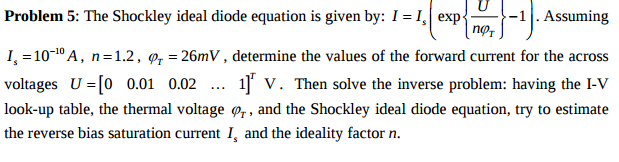
\includegraphics[width=0.7\linewidth]{screenshot008}
\label{fig:screenshot008}
\end{figure}

To calculate this task, the model of Shockley diode was coded into a function:
\begin{lstlisting}
function [F]=fun_5_Shockley(x,U)
fi=0.026;

F = x(1) * (exp(U/(x(2)*fi))-1); 
end
\end{lstlisting}


After projection of the data to the \textbf{I} current values, it was possible to use Octave curve fitting:
\begin{lstlisting}
x_est = lsqcurvefit(@fun_5_Shockley, x0, Uvalues, Ivalues);
\end{lstlisting}
The result of curve fitting is quite promising. For x = [1.0540e-09, 1.1924e+00], we obtained:
\begin{figure}[h]
\centering
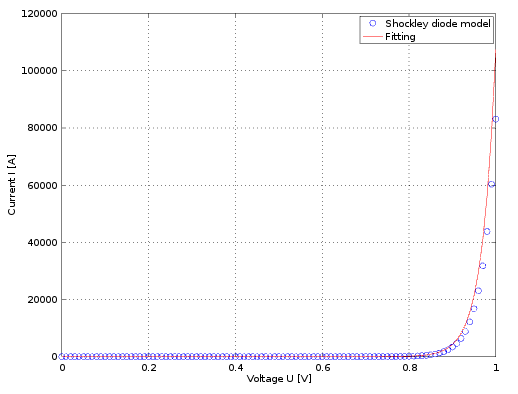
\includegraphics[width=0.9\linewidth]{screenshot009}
\caption{Curve fitting (LS) with Octave.}
\label{fig:screenshot009}
\end{figure}

\clearpage
\chapter{Listings of algorithms}
\section{Coded selected algorithms}
Algorithm 1 - Newton algorithm\\ 
\begin{lstlisting}
function [x,k] = newton(fun,x,err)
	stop = 2*err;
	iter = 0;
	while stop > err
		[F,J] = fun(x);
		dx = J\(-F);
		x = x+dx;
		[F,J] = fun(x);
		stop = max(abs(F));
		iter = iter + 1;
	endwhile
	
	iteration = iter
endfunction
\end{lstlisting}
\newpage
Algorithm 2 - Broyden method\\
\begin{lstlisting}
function [xv,it]=broyden(f,x,tol,n)
	
	fr=zeros(n,1); it=0; xv=x;
	
	Br=eye(n);
	fr=f(xv);
	
	while norm(fr)>tol
		it=it+1;
		pr=-Br*fr;
		tau=1;
		
		xv1=xv+tau*pr; 
		xv=xv1;
		
		oldfr=fr; 
		fr=f(xv);
		
		%Update approximation to Jacobian using Broydens formula
		y=fr-oldfr; 
		oldBr=Br;
		oyp=oldBr*y-pr; 
		pB=pr'*oldBr;
		
		for i=1:n
			for j=1:n
				M(i,j)=oyp(i)*pB(j);
			end;
		end;
		Br=oldBr-M./(pr'*oldBr*y);
	end;
endfunction
\end{lstlisting}
\begin{thebibliography}{8}
\addcontentsline{toc}{chapter}{Bibliography}
%\addcontentsline{toc}{section}{Literatura}
\bibitem{nocedal}
J. Nocedal, S. J. Wright, Numerical Optimization, Springer, 1999,
\bibitem{zdunek}
Zdunek R., Optimization Methods - lecture slides.
\bibitem{mathworks}
Mathworks webpage, "Unconstrained Optimization Algorithms", https://www.mathworks.com/help/optim/ug/unconstrained-nonlinear-optimization-algorithms.html
\bibitem{uni}
Nonlinear Programming course webpage, North Carolina State University,
http://www4.ncsu.edu/~kksivara/ma706/
\end{thebibliography}

\end{document}

